\documentclass{beamer}

\usepackage{fontspec,xunicode,xltxtra}

\usepackage{tikz}

\XeTeXlinebreaklocale "zh"
\XeTeXlinebreakskip = 0pt plus 1pt minus 0.1pt

%\setmainfont[Mapping=tex-text]{AR PL UMing CN:style=Light}
%\setmainfont[Mapping=tex-text]{AR PL UKai CN:style=Book}
%\setmainfont[Mapping=tex-text]{WenQuanYi Zen Hei:style=Regular}
%\setmainfont[Mapping=tex-text]{WenQuanYi Zen Hei Sharp:style=Regular}
%\setmainfont[Mapping=tex-text]{AR PL KaitiM GB:style=Regular} 
%\setmainfont[Mapping=tex-text]{AR PL SungtiL GB:style=Regular} 
%\setmainfont[Mapping=tex-text]{WenQuanYi Zen Hei Mono:style=Regular} 

\newfontfamily\hei{WenQuanYi Micro Hei}
\newfontfamily\whei{WenQuanYi Zen Hei}
\newfontfamily\kai{AR PL UKai CN}
\newfontfamily\song{AR PL UMing CN}
\newfontfamily\bhei{cwTeXHeiBold}
%\newfontfamily\lishu{SIMLI}
\setmainfont[Mapping=tex-text]{WenQuanYi Micro Hei}
\setsansfont[Mapping=tex-text]{AR PL UKai CN}
\setmonofont[Mapping=tex-text]{WenQuanYi Zen Hei Mono}

\renewcommand{\baselinestretch}{1.25}


\mode<presentation>
{
  \usetheme{Darmstadt}

 % \usetheme{Warsaw}
  % or ...
%  \usetheme{default}

  \setbeamercovered{transparent}
  % or whatever (possibly just delete it)
}


\usepackage[english]{babel}
% or whatever

%\usepackage[latin1]{inputenc}
% or whatever

\title[Beamer + xelatex] % (optional, use only with long paper titles)
{\Huge 数学软件: 应用数学家应该如何使用计算机}

\subtitle
{第一讲: 进入真正的计算机世界} % (optional)

\author[Wang HY] % (optional, use only with lots of authors)
{王何宇}
% - Use the \inst{?} command only if the authors have different
%   affiliation.

\institute[ZJU] % (optional, but mostly needed)
{
  浙江大学数学科学学院\\
  信息与计算科学系
}
% - Use the \inst command only if there are several affiliations.
% - Keep it simple, no one is interested in your street address.

\date[] % (optional)
{2022年6月}


% If you have a file called "university-logo-filename.xxx", where xxx
% is a graphic format that can be processed by latex or pdflatex,
% resp., then you can add a logo as follows:

\pgfdeclareimage[height=1cm]{university-logo}{../images/zju.jpg}
\logo{\pgfuseimage{university-logo}}

% Delete this, if you do not want the table of contents to pop up at
% the beginning of each subsection:
%\AtBeginSubsection[]
%{
%  \begin{frame}<beamer>{Outline}
%    \tableofcontents[currentsection,currentsubsection]
%  \end{frame}
%}


% If you wish to uncover everything in a step-wise fashion, uncomment
% the following command: 

%\beamerdefaultoverlayspecification{<+->}


\begin{document}

\begin{frame}
 \titlepage
\end{frame}
\begin{frame}{提纲}
  \tableofcontents
  % You might wish to add the option [pausesections]
\end{frame}

\section{引言}

\begin{frame}{自我介绍}
  \begin{itemize}
  \item 王何宇, 浙江大学数学科学学院, 信息与计算科学系.
  \item email: wangheyu@zju.edu.cn
  \item 手机: 13456940632
  \item 我承担很多信息与计算方向的专业课程, 所以大概率会和大家共事 3 年甚至更多.
  \end{itemize}
\end{frame}

\begin{frame}{本课主要内容}
  \begin{itemize}
  \item<1-> 著名的数学软件如 Matlab, Mathematica, R ...
  \item<2-> 这些我们不学!
  \item<3-> 如何优雅地用计算机做数学研究和相关的事情.
  \item<4-> 编写数学软件所需要的基础知识和技能.
  \item<5-> 编程除外...
  \item<6-> 当然, 数学也除外...
  \item<7-> 这是一门给数学人准备的非数学课.
  \end{itemize}
\end{frame}

\begin{frame}{为什么是 Linux?}
  \begin{itemize}
  \item<1-> Linux 是给正经人用的, 数学人都是正经人, 至少在做数学的时候... 
  \item<2-> 人不要去做机器该做的事, 更加不能做迁就机器的事.
  \item<3-> 除非能提高工作或思考的效率, 否则拒绝任何不必要的界面和约束. 
  \item<4-> 公开, 共享和同行评议是科学社区的基础, 也是开源社区的基础.
  \item<5-> 作为一个靠谱的数学院, Linux 将是除纯粹数学方向以外同学在未来专业课程中的生存技能.
  \end{itemize}
\end{frame}

\begin{frame}{学习本课的基本条件}
  \begin{itemize}
  \item<1-> 一个可以正常运行的 Linux 系统, 可以是独立系统, 双系统, 云主机, 或虚拟机.
  \item<2-> 能正确使用键盘, 打字速度不宜太低.
  \item<3-> 心理上能接受学习 Linux 的必要性. 
  \item<4-> 准备通过大量的练习来磨练你的基本技能.  
  \item<5-> 未来计划走应用数学的发展方向.
  \item<6-> 如果以上条件不能满足, 也不准备克服, 建议立刻退课或换课, 以免浪费时间.
  \end{itemize}
\end{frame}

\section{计算机往事}

\begin{frame}{和计算机交流}
  \begin{columns}[c]
% create the column with the first image, that occupies
% half of the slide
    \begin{column}{.5\textwidth}
      \begin{itemize}
      \item<1-> 繁华下的真像: 二进制流. 
      \item<2-> 控制计算机, 而不是被控制.
      \item<3-> core 归计算机, shell 归愚蠢的人类.
      \item<4-> 掌握了 Terminal/shell, 才能真正掌握计算机(才怪).
      \end{itemize}
    \end{column}
% create the column with the second image, that also
% occupies half of the slide
    \begin{column}{.5\textwidth}
    \begin{figure}
        \centering
        \includegraphics<1->[width=0.75\textwidth]{../images/matrix.bmp}
        \includegraphics<2->[width=0.75\textwidth]{../images/matrixbin.png}
    \end{figure}
    \end{column}
\end{columns}
  %% \begin{tikzpicture}
  %%   \node (img1) {\includegraphics[height=3cm]{res/matrix.bmp}};
  %% \end{tikzpicture}
\end{frame}

\begin{frame}{文本编辑器}
  \begin{itemize}
  \item<1-> 能基本上完全用键盘控制.
  \item<2-> 适合终端和 shell 的模式, 不占用太多的软硬件和通讯资源.
  \item<3-> 能快速高效地发送和接受指令, 完成编码.
  \item<4-> 推荐: emacs, vim, vscode.
  \item<5-> 选择一款最适合你自己, 能把你的工作效率提到最高的编辑器.
  \item<6-> 如果你还是新手, 请盲从大佬.
  \item<7-> 切记一切以效率为中心, 不要对编辑器提太多不切实际的要求.
  \item<8-> 如果你不知道怎么配置你的编辑器, 用缺省配置, 或者像同行要一个配置文件. 
  \end{itemize}
\end{frame}

\section{数学写作}
\begin{frame}{如何产生漂亮的数学文章}
  \begin{tikzpicture}[remember picture, overlay]
    \node[left = 2cm, above = -0.1cm] at (current page.east) 
         {
           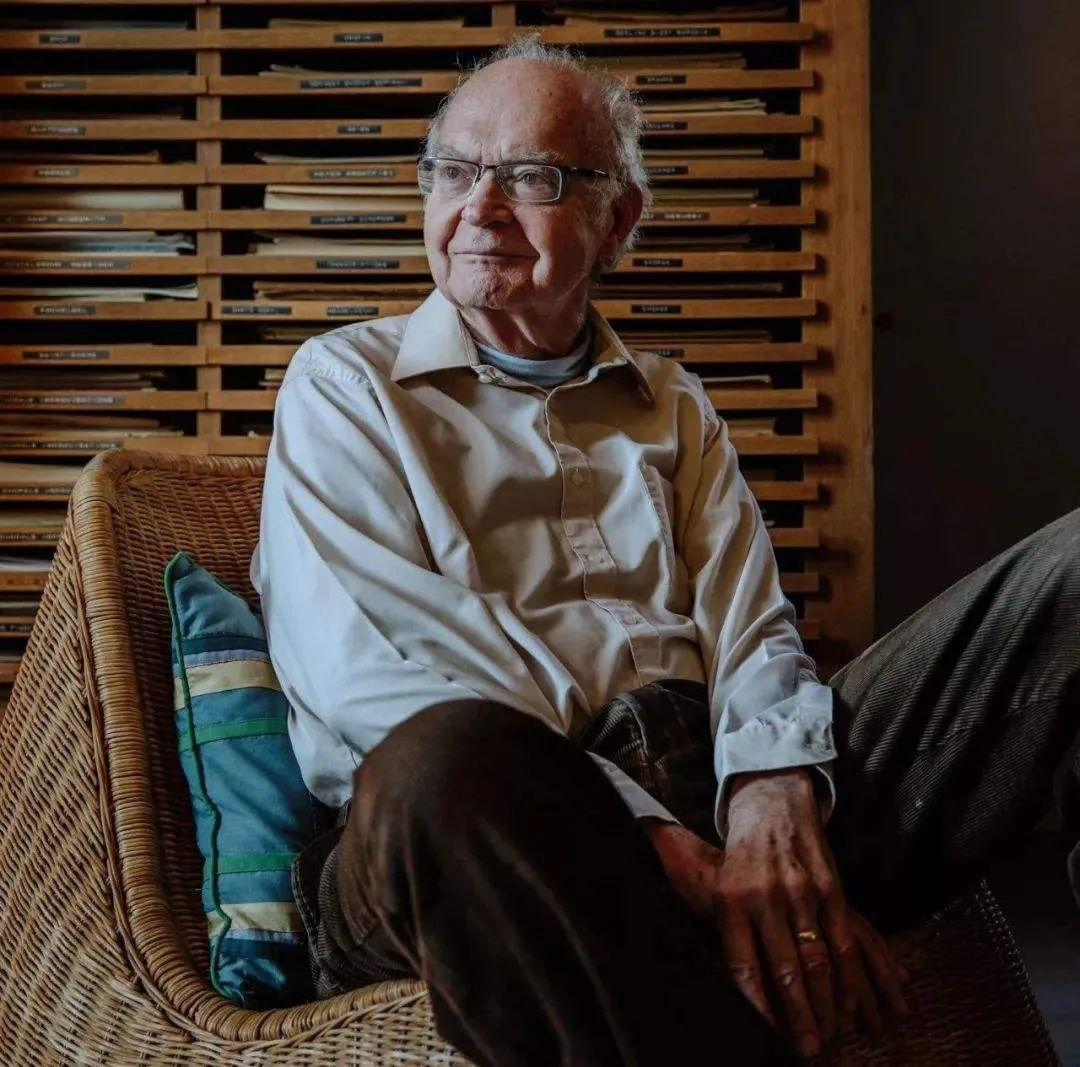
\includegraphics[width=0.25\textwidth]{../images/knuth.png}
         };
\end{tikzpicture}  
  \begin{itemize}
  \item<1-> 数学家对写作有特殊的要求.
  \item<2-> 同样必须满足键盘, 终端和高效的原则.
  \item<3-> 唯一解也是事实上的标准: \LaTeX.
  \item<4-> 参考资料: lshort, manual, ...
  \item<5-> 去找一个例子.
  \item<6-> 必须亲自动手写点什么. 
  \end{itemize}
\end{frame}

\begin{frame}{Latex进阶}
  \begin{itemize}
  \item<1-> 交叉引用和计数器.
  \item<2-> 图, 表和正文混排.
  \item<3-> 报告的制作.
  \item<4-> 手工绘图.
  \end{itemize}
\end{frame}

\section{今日份作业}


\end{document}


